% American Statistical Association (ASA) submission version,
% adapted for ASA journal formatting conventions.
% Content follows paper/impurity-importance.tex.
\PassOptionsToPackage{unicode}{hyperref}
\PassOptionsToPackage{hyphens}{url}
\PassOptionsToPackage{dvipsnames,svgnames,x11names}{xcolor}
\documentclass[12pt]{article}

\usepackage{amsmath,amssymb}
\usepackage[T1]{fontenc}
\usepackage[utf8]{inputenc}
\usepackage{textcomp}
\usepackage{lmodern}
\IfFileExists{upquote.sty}{\usepackage{upquote}}{}
\IfFileExists{microtype.sty}{%
  \usepackage[]{microtype}
  \UseMicrotypeSet[protrusion]{basicmath}
}{}
\usepackage{xcolor}
\setlength{\emergencystretch}{3em}
% Paragraph headings (Practical implications, Proposition, ...) stay
% unnumbered, as in the main build: secnumdepth 3 covers section,
% subsection and subsubsection only.
\setcounter{secnumdepth}{3}

\usepackage{longtable,booktabs,array}
\usepackage{calc}
\usepackage{etoolbox}
\usepackage{graphicx}
\usepackage{enumitem}
\makeatletter
\def\maxwidth{\ifdim\Gin@nat@width>\linewidth\linewidth\else\Gin@nat@width\fi}
\def\maxheight{\ifdim\Gin@nat@height>\textheight\textheight\else%
\Gin@nat@height\fi}
\makeatother
\setkeys{Gin}{width=\maxwidth,height=\maxheight,keepaspectratio}
\makeatletter
\def\fps@figure{htbp}
\makeatother

% ASA template page geometry --- do not change.
\setlength{\textwidth}{6in}
\setlength{\textheight}{9in}
\setlength{\topmargin}{-0.5in}
\setlength{\evensidemargin}{0in}
\setlength{\oddsidemargin}{0in}

\usepackage{caption}
\usepackage[]{natbib}
\bibliographystyle{apalike}
\usepackage{bookmark}
\IfFileExists{xurl.sty}{\usepackage{xurl}}{}
\urlstyle{same}
\hypersetup{
  pdftitle={On the misinterpretation of variable importance as effect size},
  pdfkeywords={random forests, mean decrease in impurity, Gini index, partial
  dependence, interpretability},
  colorlinks=true,
  linkcolor={blue},
  filecolor={Maroon},
  citecolor={Blue},
  urlcolor={Blue}}

\graphicspath{{../../figures/}}
\newcommand{\code}[1]{\texttt{#1}}

% \anon is ``1'' for the full manuscript and ``0'' for the anonymized
% main document that ASA reviews. The default here is 1; `make asa-anon'
% builds the 0 version without editing this file, by predefining \anon on
% the latexmk command line (see the Makefile).
\ifdefined\anon\else\newcommand{\anon}{1}\fi

% Keep the author out of the PDF metadata in the anonymized build --- an
% anonymized body is not anonymous if pdfauthor still names the author.
\if1\anon\hypersetup{pdfauthor={Christian Theil Have}}\fi

\begin{document}

\def\spacingset#1{\renewcommand{\baselinestretch}%
{#1}\small\normalsize} \spacingset{1}

%%%%%%%%%%%%%%%%%%%%%%%%%%%%%%%%%%%%%%%%%%%%%%%%%%%%%%%%%%%%%%%%%%%%%%%%%%%%%

\if1\anon
{
  \title{On the misinterpretation of variable importance\\ as effect size}
  \author{Christian Theil Have}
  \maketitle
} \fi

\if0\anon
{
  \bigskip
  \bigskip
  \bigskip
  \begin{center}
    {\LARGE\bf On the misinterpretation of variable importance as effect size}
  \end{center}
  \medskip
} \fi

\bigskip
\begin{abstract}
Impurity-based variable importance (mean decrease in impurity) is the default,
cheapest way to read which features matter in a random forest regression, and it
is routinely misread as an effect size comparable to a linear-model coefficient.
What it actually estimates is each feature's contribution to the variance of the
response: for a linear effect, the square of the coefficient times the feature's
variance. Through controlled experiments we show that importance (i) grows with
the \emph{square} of a linear coefficient; (ii) assigns an interaction's
variance to the interacting variables, so a feature with no effect of its own
can top the ranking; and (iii) gives \emph{identical} scores to a genuinely
non-linear effect and to a linear effect on a skewed feature. These problems are
distinct from the long-known bias towards features with many distinct values.
Our closing point is that they cannot be escaped by switching measure:
bias-corrected impurity, permutation importance, and SHAP-based importance
scores all inherit them, because no importance measure that reduces a feature to
a single number can separate the \emph{shape} of its effect from the
\emph{spread} of its values; partial-dependence plots, which show the effect's
shape, can. An LLM-assisted screen of literature citing the popular random
forest library \emph{ranger} suggests that one in six papers interpreting an
impurity ranking rely on it without corroboration, including heavily-cited work.
\end{abstract}

\noindent%
{\it Keywords:} random forests; mean decrease in impurity; Gini index;
partial dependence; interpretability
\vfill

\newpage
\spacingset{2}

\section{Background}
\label{sec:background-strands}

To interpret random forests it is common to calculate an variable importance measure in a similar vein to how a linear model regression estimates effect size. A commonly used measure of variable importance in random forest is the \emph{impurity importance}.
In this paper we introduce a series of experiments demonstrating how impurity importance differs from effect sizes in various regression settings. The motivation for this is that it is common (bad) practice interpret impurity performance as if it was a per-unit effect size. We demonstrate this through an LLM-based screening published articles that utilizes impurity performance to drive conclusions about effects without adequate additional corroboration.

In decision tree algorithms, a node's impurity measures the variability of the target variable among the samples reaching that node. 
For a random forest \citep{breiman2001}, the impurity importance of a feature is
the total decrease in node impurity attributable to splits on that feature,
summed over all splits and all trees \citep{breiman1984,louppe2013}. 
%
Formally, the Mean-Decrease-in-Impurity (MDI) for feature $j$ is defined as the decrease in node impurity across all splits on that feature, averaged over all trees:

\begin{equation}
\text{MDI}_j = \frac{1}{T}\sum_{t=1}^{T} \sum_{v \in S_j^{(t)}} p(v) \Delta i(v)
\end{equation}

\noindent
where $T$ is the number of trees, $S_j^{(t)}$ is the set of internal nodes in tree $t$ that split on feature $j$, $p(v)$ is the proportion of samples reaching node $v$, and $\Delta i(v)$ is the decrease in impurity (e.g., Gini or variance) caused by the split at node $v$.

This paper focus on effects of impurity importance in a regression setting.
For
regression, \code{ranger} \citep{wright2017}
(and most implementations) score a split by how much it reduces the sum of
within-child \textbf{response variances}. Note that 
for classification the impurity is the
Gini index, which measures the same thing: since $\mathbf{1}\{Y=k\}$ is
Bernoulli with variance $p_k(1-p_k)$,
$1 - \sum_k p_k^2 = \sum_k \mathrm{Var}(\mathbf{1}\{Y = k\})$, the total variance
of the class indicators. 
%Impurity importance is a variance-explained quantity in
%both settings, and that is the source of every effect studied here.
Hence, the underlying metric is variance in both regression and classification settings, impurity importance is fundamentally a variance-explained quantity. 

Two strands of prior work bear on this. The first documents that MDI is
\emph{biased} toward continuous and high-cardinality
features \citep{strobl2007,nembrini2018}; \citet{nembrini2018} give the
bias-corrected ``actual impurity reduction'' (AIR), exposed by \code{ranger} as
\code{impurity\_corrected}; further debiased MDI variants \citep{li2019,zhou2021}
address the same type bias. The second is theoretical: \citet{louppe2013}
decompose asymptotic MDI into per-variable contributions (for totally
randomised trees on categorical inputs), and \citet{scornet2023} proves that for
additive regression with independent uniform inputs, fitted with
\emph{truncated} (not fully grown) trees, MDI recovers a
\emph{variance-explained} decomposition, each
feature's score tracking $\mathrm{Var}(f_j(X_j))$, which for a linear term is
$\beta_j^2\,\mathrm{Var}(X_j)$. \citet{gromping2009} had already set
random-forest importances beside the $R^2$-decomposition importances of linear
regression, the comparison this paper makes throughout; and on the permutation
side, \citet{benard2022} show that mean decrease in accuracy is inconsistent
under dependence and give the Sobol-MDA, a consistent estimator of the total
Sobol index --- under independence, the same variance contribution normalised
by $\mathrm{Var}(y)$.

Our results are consequences of the \citet{scornet2023} identity, not new biases. 
Their value is
to show, among uncorrelated features that are all of one kind --- all continuous,
or all binary, so that a bias between feature types cannot separate them --- how
far a variance-contribution measure departs from a per-unit effect size, and that it
\emph{provably cannot} separate an effect's shape from a feature's distribution.
The new contribution is thus the sharp skew-versus-nonlinearity demonstration and
an estimate (Sections~\ref{sec:prevalence-method}--\ref{sec:prevalence-results})
of how often the misreading reaches published conclusions.

All experiments use \code{ranger} 0.18.0; the code that generates them and the
figures is available with the rest of the supporting material
(Section~\ref{sec:availability}). Unless noted, importances are the plain
\code{impurity} measure (the one the definition above describes);
Section~\ref{sec:linear} compares it against \code{impurity\_corrected}.

\subsection{Linear effects: importance is in squared-coefficient units}
\label{sec:linear}


Suppose that a random forest is fitted to the data: 
$y = a + 2b + 3c + \dots + 11k$ (11 features, coefficients $1\ldots11$)
$a,\dots,k \sim U(0,1)$, $n = 1000$.
Over seeds $1$--$10$, we regressing importance on $\beta^2$
gives a mean
$R^2$ of $0.98$ (range $0.96$--$0.99$) against $0.91$ on $\beta$ (range
$0.88$--$0.94$), and $\beta^2$ is the better fit on every seed;
Figure~\ref{fig:superlinear} shows one of them. 


\begin{figure}[htb]
\centering
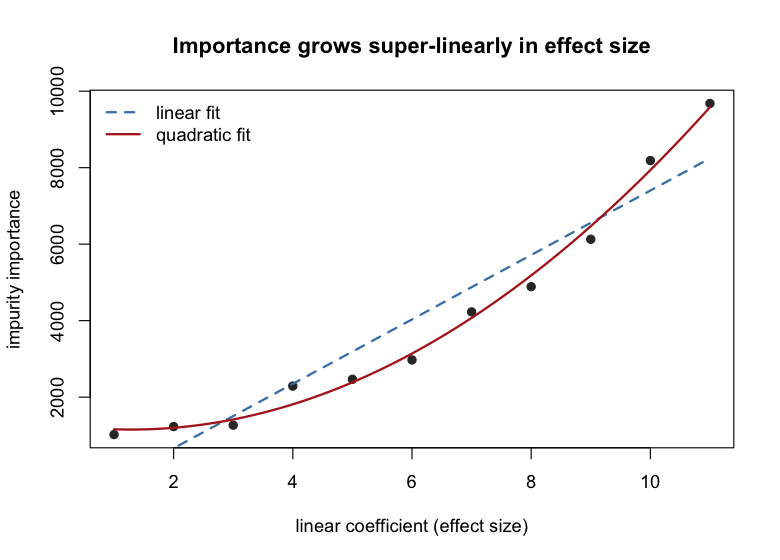
\includegraphics[width=0.95\textwidth]{fig1_superlinear.png}
\caption{Impurity importance against the coefficient $\beta$ (left, curved) and
against the variance contribution $\beta^2$ (right, linear, $R^2=0.99$).
Importance is linear in $\beta^2$, not in $\beta$.}
\label{fig:superlinear}
\end{figure}

%This empirically confirms that MDI importance is denominated in
%squared-coefficient (variance) units rather than coefficient units,
%as predicted by Scornet's identity.

For a linear term the contributed
variance is $\beta_j^2\,\mathrm{Var}(X_j)$, and here the standard-uniform
variance $\mathrm{Var}(X_j)=1/12$ is
common to all features, so the MDI should track $\beta_j^2$.

The experiment supports that, but the fit is not \emph{perfect}. This is also 
observed from the ranking of the feature importances: MDI only ranks
feature constributions correctly when they differ enough and there is enough data
to dwarf the randommness of the procedure of fitting the trees.
For this data, 
$\beta = 1\ldots11$ at the default \code{mtry}, only $3$ of $10$ seeds rank
all eleven correctly (mean Spearman $0.99$). 
AIR spreads weak features (those with smaller coefficients) further apart,
% (the $\beta = 5$ feature scores $16.4$ times the $\beta = 1$ feature, against
% $2.45$ under plain impurity, where the variance identity predicts $25$),
but it is also
far noisier from seed to seed, and the two effects offset: it ranks no better than MDI on these data
(mean Spearman $0.99$). Even where
the order holds, ``how much more'' is not comparable to a coefficient.

\subsubsection{Relative interpretations of feature importances}
An experiment that examines divergences from the expected ratios between 
variable importances enables determining in more detail how and why 
variable importances in practice differ from the theoretical expectation
of them tracking  $\beta_j^2$.
Here, 
a random forest is fitted a data where feature contributions are doubled per term: $y = a + 2b + 4c$, with
$a,b,c \sim U(0,1)$, $n = 1000$. The forest's out-of-bag (OOB) $R^2$ is $0.98$.
Impurity importance (both MDI and AIR) ranks the features in the correct
order, 
but their \emph{ratios} do not match the ordinary-least-squares (OLS)
coefficient ratios (table entries are means over seeds $1$--$10$, ranges in
parentheses):

\begin{center}
\begin{tabular}{rccc}
\toprule
feature & OLS coefficient & MDI (ratio) & AIR (ratio)
\\
\midrule
a & 1 & 1.00 & 1.00 \\
b & 2 & 2.24 (2.00--2.47) & 4.19 (2.97--5.53) \\
c & 4 & 7.19 (6.49--8.21) & 16.88 (11.06--22.94) \\
\bottomrule
\end{tabular}
\end{center}

A coefficient ratio of $1:2:4$ becomes an importance ratio of $1:2.2:7.2$ under
MDI and $1:4.2:16.9$ under AIR: the
feature ordering is correct and the growth is clearly super-linear, but the MDI spread is not
 $1:4:16$, the ratio of the \emph{squared} coefficients that Scornet's identity in 
Section~\ref{sec:background-strands} predicts. 

%For a linear term the contributed
%variance is $\beta_j^2\,\mathrm{Var}(X_j)$, and here the standard-uniform
%variance $\mathrm{Var}(X_j)=1/12$ is
%common to all features, so the MDI should track $\beta_j^2$.k

The difference 
%to this expectation
is due to the number of features drawn as
candidates at each node (a configurable parameter called \code{mtry}), intended
to decorrelate the trees. In \code{ranger} it defaults
to $\lfloor \sqrt{p} \rfloor$, here $1$: each node must split on the
single feature it drew, so $a$ takes splits it would never win in competition
and
is inflated at the expense of $c$. Letting features compete removes the dilution
(means over seeds $1$--$10$, $n=1000$, 500 trees):

\begin{center}
\begin{tabular}{clc}
\toprule
\code{mtry} & MDI (ratio) & \\
\midrule
1 (default at $p=3$) & $1:2.25:7.26$ & compressed \\
2                    & $1:3.93:15.5$ & $\approx$ predicted $1:4:16$ \\
3 ($=p$, no split randomisation) & $1:4.45:19.1$ & overshoots \\
\bottomrule
\end{tabular}
\end{center}

At $\code{mtry}=p$ the
strongest feature wins the root split in every tree, and overshoots. Tree depth
matters too, but not in the direction Scornet's truncated-tree condition might
suggest. He proves the identity for truncated trees and warns that fully grown
trees yield positively biased MDI \citep{scornet2023}, and explains that the
bias comes from fitting the noise term; $y$ here is noiseless, so it cannot
operate. A sweep limiting the maximal depth of trees
%\code{max.depth} sweep (seeds $1$--$10$) 
shows the opposite, finite-sample
effect: truncating the trees removes splits, and the features with the smallest
variance contributions are the first to lose them. At depth $2$ with
$\code{mtry}=p$
the weakest feature earns no splits at all. Deepening lowers the ratios in
both settings: at $\code{mtry}=p$ they approach the predicted $1:4:16$
($1:12.0:58.3$ at depth $4$, $1:4.45:19.1$ fully grown), and at the default
$\code{mtry}=1$ they fall further below it ($1:3.38:12.1$ at depth $2$,
$1:2.25:7.26$ fully grown). The residual overshoot at $\code{mtry}=p$ is a
finite-sample effect: it diminishes as $n$ grows
($1:4.15:17.1$ at $n=4000$, $1:4.01:16.1$ at $n=64000$; means over seeds
$1$--$10$). This is aligned with Scornet's theorem about greedy CART splitting
being asymptotic in $n$. The compression at $\code{mtry}=1$, which the theorem
does not
cover, also shrinks with $n$ but far more slowly ($1:3.51:13.7$ at
$n=64000$). The deviations in the table are finite-sample properties of the
fitting procedure --- split randomisation and greedy split selection --- and
shrink toward the squared-coefficient prediction as $n$ grows.

%The AIR bias correction behaves differently. 
%It
%pairs each feature with a reordered copy of itself --- same distribution,
%same number of split points, no relationship to the response --- and
%subtracts the variance reduction that copy earns from the feature's own.
%It is therefore a difference of variance reductions, expressed in units of
%variance, and no closer to a per-unit effect size than plain impurity.
%
Compared to MDI, AIR is nearly
\code{mtry}-insensitive: averaged over 10 randomly seeded experiment runs, its ratios are
$1:4.2:16.9$ at the
default, $1:4.0:16.0$ at $\code{mtry}=2$, and $1:4.1:16.7$ at $\code{mtry}=3$,
near the predicted $1:4:16$ throughout.
%
%The price is sampling variance, and it comes from that same subtraction.
Note, the AIR formula includes and additional term (a re-ordered copy of the feature) compared to MDI which 
substracts the reordered variance reduction from the features own.
In this experiment, for the weakest feature the two terms in AIR nearly cancel, leaving a small difference
between two large numbers, so the ordinary noise each carries falls on a much
smaller result: feature $a$'s AIR varies about three times as much from seed to
seed as plain impurity's ($27\%$ against $10\%$ relative standard deviation).
The strongest feature, where the subtraction takes little off the total, stays
steady at $6\%$. Since the unstable feature is the one the ratio divides by,
AIR's $c$ ratio spans $11.1$--$22.9$ over the ten seeds against $6.5$--$8.2$
for plain impurity. The increased sampling variance suggest that AIR ratios 
are readable only as an average over seeds.

%\paragraph{Takeaway.}
%Furthermore, an interaction lets a variable with no marginal effect outrank one
%that has
%(Section~\ref{sec:interactions}), and unequal feature distributions reorder
%the ranking on their own (Section~\ref{sec:confound}).

\paragraph{Practical implications.} Read an impurity ranking as an ordering
among comparably distributed features, and expect inversions where
contributions are close. Its ratios are in squared-coefficient units and
further compressed by the default \code{mtry}, so a bar twice as tall does not
mean an effect twice as large. AIR was built to remove the bias
toward null and high-cardinality features, but for continous features, it also follows the
variance contribution more closely than plain MDI, but varies far more from seed to seed on
weak features; average it over seeds before reading a ratio from it.

\subsection{Interactions}
\label{sec:interactions}

Random forests are particularly adept at capturing interactions between
features and are
for that reason often utilized when the features are believed to interact.
Here, we examine how variable importances are allocated when a feature is
itself an interaction between other features.

Consider a pure two-way parity interaction with no marginal effects:
\[
  y = c/10 + \big((a + b) \bmod 2\big), \qquad a,b,c \in \{0,1\}, \quad n =
  10000.
\]
Neither $a$ nor $b$ carries information about $y$ on its own; only their joint
parity does. $c$ is the only variable with an independent effect. We fit a
random forest and a linear regression model against this data.

Main-effects \textbf{OLS} sees only $c$: the fitted coefficients on $a$ and $b$
are $0.000$ and $0.000$ against $0.101$ for $c$, at $R^2 = 0.01$.
For binary inputs $(a+b) \bmod 2 = a + b - 2ab$ is bilinear, so adding an
$a{\times}b$ term fits the target exactly ($R^2 = 1.000$).

When the interaction is captured in the Random Forest, the two interacting
variables $a$ and $b$
are allocated most of the variable importance. The size of their share follows
from the variance decomposition. Impurity importance sums the reduction in node
sum of squares over splits, and
trees grown to purity remove $n\,\mathrm{Var}(y)$ between them, so the
importance
divides as the variance does. The target is additive in two independent pieces,
$\mathrm{Var}(c/10) = 0.0025$ and $\mathrm{Var}\big((a+b) \bmod 2\big) = 0.25$:
the
coefficient $1/10$ gives $c$ one hundredth of the pair's variance, so $c$ gets
importance
$1\%$ and the pair $99\%$. Note that this is exactly the explained
variance ($R^2 = 0.01$) of main effects OLS.
At $\code{mtry} = 3$, the measured total is $2525.2 = n\,\mathrm{Var}(y)$ and
$c$ receives $1.02\%$
of it. Over seeds $1$--$10$ at the default $\code{mtry} = 1$, $a$ and $b$
average
$451$ (SD $29$) against $15$ for $c$, and its share rises to $1.6\%$, because
$\code{mtry} = 1$ truncates trees and the loss falls harder on the pair, whose
credit needs both variables on one path: a node whose single candidate is
already constant becomes terminal, so paths are cut before both $a$ and $b$
have been split on. Figure~\ref{fig:interaction} shows the contrast
against main-effects OLS.

Since $a$ and $b$ are exchangeable by construction, any difference between their
importances is sampling noise, and within a single seed they spread by
$2$--$20\%$ (median $10\%$), against $1$--$6\%$ when the parity is replaced by
equal \emph{marginal} effects for $a$ and $b$ ($y = c/10 + (a + b)/2$).
So only the $a,b \gg c$ gap is informative here.

The interaction spread is the wider one because credit for an interacting
variable is
conditional on tree topology. Splitting on $a$ or $b$ alone reduces no variance;
once a tree has split on one of the pair, the
other separates the parity completely. Each tree therefore hands the pair's
entire contribution to whichever variable it splits last.
At $\code{mtry} = 1$ that division between $a$ and $b$ is made by the
candidate draw rather than by the data,
so the number of trees crediting each variable is binomial and the imbalance
averages
away as trees accumulate.
At
$\code{mtry} = p$ both variables compete at each node and the one with the
larger
empirical decrease wins:
with bagging disabled the pair's credit goes entirely to one variable, and
bootstrap resampling only partly decorrelates that choice.
Conditional on the
training sample the surviving imbalance therefore becomes a bias rather than
noise:
every tree re-derives the same allocation from the same data, so averaging
converges to that allocation instead of to an even split. Refitting each of six
datasets with
eight forest seeds at $\code{mtry} = p$ confirms this: all eight land on the
same side of an even split for every dataset, and from $500$ to $4000$ trees the
forest-to-forest SD falls from $0.02$ to $0.005$ while the mean does not move.
The size of the imbalance is the sample's: the $a$-vs-$b$ spread runs from
$3\%$ to $119\%$ across the six.

Breiman introduced the per-node
random draw of $F$ candidate inputs (what the parameter \code{mtry} implements)
because
``the randomness injected has to minimize the correlation $\bar\rho$ while
maintaining strength'' \citep[\S3; Thm.~11.2 for regression]{breiman2001},
$\bar\rho$ being the correlation between the predictions of pairs of trees.
At $\code{mtry} = p$ none of that randomness is injected. The $\code{mtry}$
setting that results in the best OOB generalization (OOB $R^2$ $1.00$ at
$\code{mtry} = p$ against $0.59$ at the default) is therefore also the one whose
division of
importance between $a$ and $b$ is least trustworthy.

AIR was not designed to remove \emph{this bias}, but it has an incidental
effect through tree decorrelation.
At $\code{mtry} = 1$ the two importance measures are indistinguishable, whereas
AIR shows improvement
at $\code{mtry} = p$ (median $a$-vs-$b$ spread $13.3\%$ against $29.1\%$).
This comes
from its permuted pseudo-variables enlarging the candidate pool to $2p$, which
lowers $\bar\rho$ in the same vein as a smaller \code{mtry} would, degrading
also
OOB $R^2$ to $0.946$.

The same allocation question can be put to the two measures most often used to
corroborate an impurity ranking, and which this paper takes as its foils:
\textbf{permutation importance} (OOB Breiman-style, as returned by
\code{ranger}) and \textbf{mean absolute TreeSHAP} ($\overline{|\varphi_j|}$,
the path-dependent \emph{observational} variant). Both confirm the $a,b \gg c$
reading, so switching measure does not rescue the interpretation, and both give
$a$ and $b$ equal scores. They part company on how the pair's shared credit is
divided. Permutation importance charges each member the \emph{entire}
interaction rather than a share of it --- scrambling either variable destroys
the whole parity --- so the pair's importances sum to twice the interaction
variance, while mean $|\varphi|$ partitions the credit exactly. Each is
denominated in units of its own, so neither is an effect size.
Appendix~\ref{app:interactions} derives both; Table~\ref{tab:interactions}
collects the allocations.

\begin{table}[htb]
\centering
\caption{The four allocations on the seed-42 parity dataset, ratios normalised
to $c$ (the only variable with a marginal effect).}
\label{tab:interactions}
\begin{tabular}{llccc}
\toprule
\code{mtry} & measure & $a : b : c$ (to $c$) & $c$ share & $a/(a{+}b)$ \\
\midrule
1 (default) & MDI              & $28 : 23 : 1$    & $1.9\%$  & $0.545$ \\
            & AIR              & $21 : 22 : 1$    & $2.3\%$  & $0.496$ \\
            & permutation      & $53 : 53 : 1$    & $0.9\%$  & $0.501$ \\
            & mean $|\varphi|$ & $2.7 : 2.7 : 1$  & $15.8\%$ & $0.500$ \\
\midrule
3 ($= p$)   & MDI              & $44 : 52 : 1$    & $1.0\%$  & $0.459$ \\
            & AIR              & $40 : 39 : 1$    & $1.2\%$  & $0.503$ \\
            & permutation      & $100 : 100 : 1$  & $0.5\%$  & $0.500$ \\
            & mean $|\varphi|$ & $5 : 5 : 1$      & $9.1\%$  & $0.500$ \\
\bottomrule
\end{tabular}
\end{table}

\paragraph{Practical implications.} A variable at the top of an impurity
ranking may have no marginal effect at all and owe its place to an interaction,
and switching measure does not rescue the reading: permutation importance and
mean $|\varphi|$ rank the interacting pair as far above $c$ as MDI does, while
within an interacting pair, the order is not to be read --- the division of
their shared credit is candidate-draw noise at the default \code{mtry} and a
sample-fixed bias at $\code{mtry} = p$ under MDI, and permutation importance
additionally charges each member the full joint effect rather than a share of
it.
What distinguishes the two cases is the one-way
partial-dependence plot (PDP) under a tall bar: here it is flat, and the parity
appears only in the joint PDP over $(a,b)$.

\begin{figure}[htb]
\centering
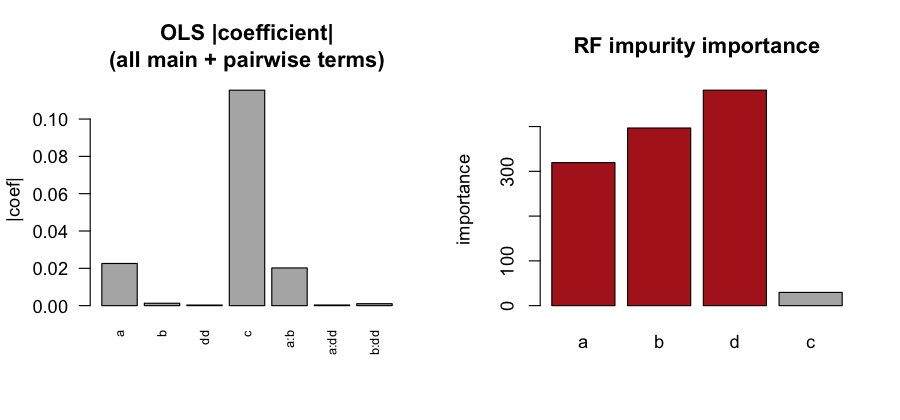
\includegraphics[width=0.85\textwidth]{fig2_interaction.png}
\caption{Same data, two views. Main-effects OLS assigns $a$ and $b$ essentially
zero coefficient, seeing only $c$; RF impurity importance ranks the two
interacting variables far above it. The ordering between $a$ and $b$ is sampling
noise --- they are exchangeable by construction.}
\label{fig:interaction}
\end{figure}

\subsection{What the split criterion sees, and what it discards}
\label{sec:variance}

Two properties of variance-based splitting underlie the effects in the sections
that follow. Take a
noise-free, sorted dataset and sweep every single split, scoring each by the sum
of within-child variances, for $y = x$, $y = x^2$, $y = x^3$ ($x =
1\ldots1000$):

\begin{center}
\begin{tabular}{cccc}
\toprule
response & min split-variance & fraction of parent variance removed & argmin split index (1--1000) \\
\midrule
$x$   & $4.2 \times 10^{4}$  & $0.75$ & 500 (centre) \\
$x^2$ & $4.3 \times 10^{10}$ & $0.76$ & 697 \\
$x^3$ & $4.1 \times 10^{16}$ & $0.74$ & 799 \\
\bottomrule
\end{tabular}
\end{center}

Here \code{argmin} is the position among the $1000$ sorted values of $x$ at
which the split minimizes the sum of within-child variances.

The raw minimum grows by orders of magnitude with the degree, but that is a
\emph{response-scale artifact}: as a fraction of parent variance removed, all
three splits are essentially equal (${\approx}0.75$). The two relevant
properties that the table illustrates are:

\begin{enumerate}[leftmargin=1.6em]
\item \textbf{Trees discard feature-distribution shape.} A split compares only
the
  \emph{ordering} of a feature's values, so the tree is invariant to any
  monotone
  transform and cannot see whether a feature is uniform or heavy-tailed,
  information a per-unit effect size needs. This is the root cause of the
  confound
  in Section~\ref{sec:confound}.
\item \textbf{The optimal split migrates with response shape.} For a linear
  response the best split is central; for higher orders it moves toward the
  high-$y$ tail ($500 \rightarrow 697 \rightarrow 799$). The imbalance leaves
  more
  structure in the large child, so more splits follow down that branch, each
  charged to the same feature.
\end{enumerate}

Neither property depends on \code{mtry}: the sweep has a single feature, and
\code{mtry} decides which features compete at a node, not where a feature's
best threshold falls or what the split can see.
Impurity importance is a sum of those split scores over the fitted trees, so it
inherits both properties: it summarises variance contribution over the feature
ordering, but is blind to the metric the ordering lives on.

\section{Non-linear effects: variance contribution predicts the ranking}
\label{sec:nonlinear}

Data: $y = a + b^2 + c^3$, with $a = 1 + U_a$, $b = 1 + U_b$, $c = 1 + U_c$ and
$U_a, U_b, U_c$ independent $U(0,1)$ draws, $n = 10000$. (The draws are
\emph{separate} per feature: a single shared $U$ would make the three features
collinear and the experiment vacuous.)
Each term's variance contribution grows with its degree, so
Section~\ref{sec:background-strands} predicts
$\mathrm{vip}(a) < \mathrm{vip}(b) < \mathrm{vip}(c)$; the forest confirms it,
$1751 < 8166 < 39632$ (a $1:4.7:22.6$ ratio). A linear model still returns non-zero
coefficients, but they are uninterpretable: the residuals are visibly non-normal.

\section{Non-linearity and feature scale are indistinguishable}
\label{sec:confound}

Take equal linear effects but
skewed feature \emph{distributions}:
\[
  a = 1 + U_a, \quad b = (1 + U_b)^2, \quad c = (1 + U_c)^3, \quad y = a + b +
  c,
  \quad n = 10000,
\]
where $U_a, U_b, U_c$ are \emph{the same} draws used in
Section~\ref{sec:nonlinear}. Every feature enters with coefficient 1, and OLS
recovers $1.00, 1.00, 1.00$: nothing about the \emph{effects} is non-linear. Yet
the forest reports \textbf{1751 / 8166 / 39632}, a $1:4.7:22.6$ spread
--- exactly the same as the non-linear model of
Section~\ref{sec:nonlinear} (Figure~\ref{fig:confound}).

The agreement is exact because the two datasets present the forest with the
same information: the same response vector, and each feature in the same
order. The following proposition makes this precise.

\paragraph{Proposition.} Fix draws $U_a, U_b, U_c$ and compare two worlds:
\emph{(A)} features $(1{+}U_a,\; 1{+}U_b,\; 1{+}U_c)$ with response
$y = a + b^2 + c^3$, and \emph{(B)} features
$(1{+}U_a,\; (1{+}U_b)^2,\; (1{+}U_c)^3)$ with response $y = a + b + c$. Then
the
response vector is the same in both worlds, and each world-B feature is a
strictly increasing transform of its world-A counterpart. If (i) bootstrap
indices and candidate-feature draws are held fixed across the two fits, and
(ii) split selection depends on a feature only through the \emph{ordering} of
its values --- as it does for an exhaustive search over thresholds between
consecutive order statistics, \code{ranger}'s default
\code{splitrule = "variance"} --- then the two forests are identical tree for
tree as partitions of the in-bag sample, and every importance that is a
functional of those partitions (MDI,
AIR) coincides exactly.

Equal variance contribution is a by-product of the same construction; the
argument does not use it.

Both hypotheses can fail in practice. Hypothesis (i) fails in any script that
fits the two worlds one after the other without reseeding, and the cross-world
variation that follows is seed noise: world B under any RNG state gives the same
trees as world A under that state, so an unseeded cross-world pair is
distributed exactly as refitting a single world under two seeds. A sweep over
seeds $1$--$10$ confirms the corollary in \code{ranger}'s implementation: the
identity is exact at every seed, and across all $\binom{10}{2} = 45$ pairs of
distinct seeds the cross-world gap equals the same-world gap.
Hypothesis (ii) concerns the split search: a rule that sees a feature only
through the ordering of its values discards exactly the distribution-shape
information that would tell the two worlds apart.
\code{splitrule = "extratrees"} keeps a little of it, drawing thresholds
uniformly from the feature's value \emph{range} instead of scanning order
statistics. Squaring stretches that range, so the same draw lands elsewhere in
the data and the two worlds separate: $1:4.9:23.7$ against $1:5.0:24.6$.
The same thing happens to predictions. \citet{galili2016} show that a tree's
predictions for new observations are not invariant to monotone transforms of its
features, for the same reason: a threshold placed between two observed values
sits at their midpoint, and stretching the scale moves that midpoint even though
the training points either side of it stay put.

This is \textbf{not specific to impurity}, and debiasing does not touch it.
Bias-corrected impurity (AIR), permutation importance, and global mean
$|\text{SHAP}|$ all give the same ratios in both worlds:

\begin{center}
\begin{tabular}{lcc}
\toprule
measure & ratio & cross-world agreement \\
\midrule
impurity (MDI)            & $1:4.7:22.6$   & exactly $0$ \\
impurity, debiased (AIR)  & $1:8.8:47.4$   & exactly $0$ \\
permutation               & $1:9.2:50.3$   & ${\sim}10^{-4}$ \\
mean $|\text{SHAP}|$      & $1:3.06:6.98$  & $1.3 \times 10^{-4}$ \\
\midrule
standardised OLS          & $1:2.98:6.88$ (A), $1:2.99:6.98$ (B) & $1.4 \times
10^{-2}$ \\
\bottomrule
\end{tabular}
\end{center}

The first four follow from the proposition, in descending strictness. MDI is a
functional of the fitted trees alone, so it agrees identically. AIR agrees
identically for the same reason, one step removed: the correction subtracts the
impurity a permuted copy of each feature would earn, and under hypothesis (i)
those permutation draws are fixed too, while permuting commutes with monotone
transforms --- the permuted copy of $(1+U_b)^2$ is the square of the permuted
copy of $1+U_b$ --- so the correction is a functional of the same trees and the
same orderings. Debiasing moves the ratio from plain MDI's compressed
$1:4.7:22.6$ toward the variance-contribution ratio $1:9.07:48.96$ (a single
draw; Section~\ref{sec:linear} warns against reading any single-seed AIR
ratio closely and that applies here too), and moves the cross-world agreement
not at
all. Permutation and
path-dependent TreeSHAP \citep{lundberg2020} also touch feature values at the
thresholds --- one
through the values it shuffles, the other through node weights it reconstructs
from the data, which differ by at most two observations on $0.3\%$ of nodes ---
and agree to four significant figures rather than exactly.

Standardised OLS is the control. It never sees the forest, so the proposition
gives it nothing, and the two worlds are genuinely different regressions:
projecting $y$ onto $1+U$ is not projecting it onto $(1+U)^2$. The gap between
the two has a closed form. With independent features, the standardised
coefficient of $b$ is $\mathrm{sd}(b^2)/\mathrm{sd}(y)$ in world B and
$\mathrm{Cov}(b^2, b)/(\mathrm{sd}(b)\,\mathrm{sd}(y)) =
\mathrm{Corr}(b, b^2)\,\mathrm{sd}(b^2)/\mathrm{sd}(y)$ in world A, so the two
worlds differ by exactly the factor $\mathrm{Corr}(b, b^2)$: the fraction of the
squared feature that a linear projection captures. For $U(1,2)$ these
correlations are $0.9963$ for the square and $0.9861$ for the cube, and the
table reproduces them: $2.98/2.99 = 0.997$ and $6.88/6.98 = 0.986$. The
discrepancy is the population correlation gap itself, two orders of magnitude
larger than anything the proposition-pinned measures show. That a standardised
coefficient ties a variable's apparent importance to the spread of its
distribution is a long-standing complaint in the regression
literature \citep{bring1994}; the proposition is the tree-based version, with
effect shape and feature spread made exactly indistinguishable.

The spread of agreement is what identifies the mechanism. Equal variance
contribution alone would predict uniform approximate agreement, and cannot
produce an exact zero. Nor is being a variance the operative property: MDI and
permutation are denominated in variance, but mean $|\text{SHAP}|$ tracks the
\emph{square root} of the variance contribution ($\sqrt{1:9.07:48.96} =
1:3.01:7.00$), one power lower, and is confounded just the same. What the four
share, and what none of them escapes, is being a functional of the fitted model
and of the feature ordering, and the proposition makes both identical across the
two worlds. Any marginal importance inherits this,
whatever its units. The remedy is a shape-aware view: a partial-dependence plot,
or a SHAP \emph{dependence} plot, which plots each observation's SHAP value
against its feature value, and the feature values do differ between the two
worlds.

\begin{figure}[htb]
\centering
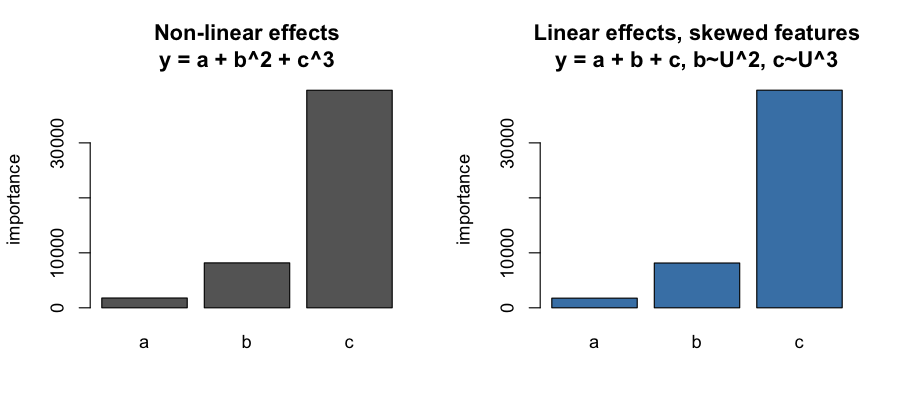
\includegraphics[width=0.85\textwidth]{fig3_confound.png}
\caption{Provably identical importances from two different worlds. Left:
genuinely
non-linear effects. Right: linear effects on skewed features. No marginal
importance measure can distinguish them.}
\label{fig:confound}
\end{figure}

\paragraph{Practical implications.} A tall importance bar can mean a strong or
non-linear effect, an interaction (Section~\ref{sec:interactions}), or merely a
heavy-tailed feature, and no marginal importance can say which --- not plain
or debiased impurity, not permutation, not mean $|\text{SHAP}|$. Switching
measure does not help; a shape-aware view does. The
partial-dependence plot \citep{friedman2001} of the skewed-feature world is a
straight line while the non-linear world's curves, at identical importances;
a SHAP dependence plot separates them the same way. The PDP averages the model
over the other features' marginal distribution, which is exact for
independent features as here; under dependence it evaluates the model on
combinations that do not occur in the data and can show its extrapolation
rather than an effect \citep{hooker2021}. There, accumulated local effects
(ALE) \citep{apley2020}, which
accumulates effects conditional on the neighbouring feature
distribution, replaces it. A SHAP dependence plot does not share this
exposure when the SHAP values are computed with path-dependent TreeSHAP, as
here: it is drawn only at observed data points, and path-dependent TreeSHAP
follows the training data down each tree rather than evaluating the model on
combinations that never occur.

\section{Prevalence in the literature}

The preceding sections establish, in controlled settings, how a
variance-contribution measure can be misread as an effect size. To estimate how
often that misreading reaches published conclusions, we screened the literature
that uses the \code{ranger} R package --- one of the most widely used
random-forest implementations, and the one whose importances these results
concern. We screen for papers whose stated conclusions depend on the magnitude or
ranking of an impurity importance without the corroboration that would guard
against the effects of Sections~\ref{sec:linear}--\ref{sec:confound}.

\subsection{Method}
\label{sec:prevalence-method}

\paragraph{Corpus.} We took every work recorded by OpenAlex as citing the ranger
reference publication \citep{wright2017} (OpenAlex work \code{W2157395790}),
$3{,}189$ works in total. For each we retrieved bibliographic metadata from
OpenAlex and, where an open-access full text was available, the full text from
Europe PMC; $773$ works had retrievable open-access full text. Screening was
restricted to these, because the detail needed to judge exposure --- which
importance measure is used, and whether it is corroborated --- is almost never
present in an abstract.

\paragraph{Relevance filter.} Many papers cite ranger only for its speed or for
prediction and never interpret a variable importance. To drop these without
discarding relevant work, we required a textual mention of variable importance: a
paper was retained if its full text matched, case-insensitively, any of the
following regular-expression alternatives.
\begin{verbatim}
(variable|feature|permutation|gini|impurity)\s+importance
importance\s+(score|value|ranking|measure)
mean decrease
decrease in (impurity|gini|accuracy)
\bMDI\b   \bMDA\b   \bBoruta\b
impurity[_\s]?corrected
most important (variable|feature|predictor)
\end{verbatim}
$524$ of the $773$ matched. The filter is deliberately broad: an earlier version
that also required a significance keyword (\code{importance\_pvalues}, Altmann,
Janitza, Boruta) missed most exposed papers. Of $40$ sampled papers it rejected,
$24$ still used an impurity importance and $11$ met the flag criterion below,
because many papers rank features by impurity importance with no significance
test. In total $544$ papers were screened: the $524$ matches plus $20$ from
earlier passes (including that probe) that the broadened filter misses. Its recall
was not separately re-estimated (see limitations).

\paragraph{Two-stage screen.} Each paper was read by a large language model under
a fixed instruction and asked to return a structured judgement; the verbatim
prompts are in the supporting repository (Section~\ref{sec:availability}). The
screen has two stages using different models, so that the second acts as an
adversarial check on the first.

\emph{Stage 1 --- screening.} A first model (Claude Haiku 4.5) read each paper and
recorded which importance measure it uses, whether it interprets that importance's
magnitude or ranking, which corroborating analyses it reports, and a flag for
whether a central conclusion could have been affected. The instruction was
explicit that the bias corrupts magnitude and ranking, not the binary verdict
that a variable is used, so a significant importance $p$-value
\citep{altmann2010,janitza2018,kursa2010}
does not by itself protect a conclusion. A paper was flagged only if it leaned on
the magnitude or ranking of an impurity importance for a central conclusion
\emph{without} corroboration, defined as permutation importance,
SHAP \citep{lundberg2017}, partial-dependence/ALE \citep{friedman2001,apley2020},
conditional importance \citep{strobl2008}, or held-out validation of the
\emph{selected} features (overall test accuracy does not count, as it validates
prediction, not the ranking). Every flag required a quoted passage.

Counting SHAP as corroboration is generous. Section~\ref{sec:confound} shows
that a global mean $|\text{SHAP}|$ ranking carries the same shape/skew confound
as impurity importance, while a SHAP \emph{dependence} plot does not, and the
screen does not distinguish the two forms, so papers reporting only a mean
$|\text{SHAP}|$ ranking were credited with corroboration they do not have. This
can only suppress flags, so it makes the confirmed count conservative.

\emph{Stage 2 --- adjudication.} Every flagged paper was independently re-read by
a second, stronger model (Claude Sonnet 5) under an explicitly adversarial
instruction: its task was to \emph{refute} the flag. It returned a verdict of
\emph{confirmed}, \emph{refuted}, or \emph{uncertain}, and confirmed only when all
three conditions held at once: 1) the paper genuinely uses an impurity (not solely
a permutation or SHAP) importance, 2) the ranking is central to a stated conclusion,
and 3) the ranking is not adequately corroborated. Both models were accessed in
July 2026. Using two models from a single vendor means the adjudication is a
precision filter, not an independent validation --- a different-vendor or human
check would be stronger; we return to this in the limitations.

\subsection{Results}
\label{sec:prevalence-results}

Table~\ref{tab:prevalence} traces the corpus through the pipeline. Of the $544$
papers screened, $307$ were judged to use an impurity importance and $125$ were
flagged in stage~1. The adversarial adjudication confirmed $55$, refuted $65$, and
could not decide for $5$, overturning roughly $56\%$ of the stage-1 flags. The
implied stage-1 precision is therefore about $44\%$, and raw screening counts
should be discounted accordingly.

\begin{table}[htb]
\centering
\caption{The ranger-citing corpus traced through the screening pipeline. The
final rows are counts of screened papers; percentages in the text are relative to
the $544$ screened.}
\label{tab:prevalence}
\begin{tabular}{lr}
\toprule
Stage & Count \\
\midrule
Works citing ranger (OpenAlex) & $3{,}189$ \\
With open-access full text & $773$ \\
Matching the relevance filter & $524$ \\
Screened (filter matches $+$ non-match sample) & $544$ \\
\midrule
Using an impurity importance (stage 1) & $307$ \\
Flagged (stage 1, Haiku 4.5) & $125$ \\
\quad Confirmed (stage 2, Sonnet 5) & $55$ \\
\quad Refuted & $65$ \\
\quad Uncertain & $5$ \\
\bottomrule
\end{tabular}

\vspace{4pt}
{\footnotesize\emph{Note:} the $544$ screened papers comprise all $524$
filter matches plus $20$ non-matching papers that were screened in earlier passes
before the filter was finalised, including the random recall sample; all $524$
filter matches were screened.}
\end{table}

Taking the confirmed count in Table~\ref{tab:prevalence} at face value, $55$ of
the $544$ screened papers state a central conclusion that could have been
distorted by the effects of Sections~\ref{sec:linear}--\ref{sec:confound} and did
not cross-check it. That is about $10\%$ of the screened papers. Measured against
the $307$ that actually interpret an impurity importance, it is $18\%$, roughly
one in six. As a share of all $773$ full-text ranger-citing works it is about
$7\%$.

Two features of the confirmed set are worth drawing out. First, exposure is
concentrated in papers that use no significance machinery: $51$ of the $55$
confirmed papers ($93\%$) report no importance $p$-value or Boruta selection and
simply rank features by impurity importance, suggesting that familiarity with
significance testing goes with more cautious interpretation of a ranking. Second,
the confirmed papers are not confined to low-visibility venues: citation counts
span the full range of the corpus (median $11$, versus a corpus median of $10$),
and $12$ of the $55$ exceed $50$ citations.

\paragraph{Limitations.} These are model judgements, not audits: a flag means a
conclusion \emph{could} have been affected and was uncorroborated, not that it is
wrong, and predictive accuracy is unaffected. The $10\%$ is an unvalidated
estimate; stage 2 raises precision but is not independent validation, and there
is no human ground truth. Only $773$ of $3{,}189$ works had open-access full
text, and open access correlates with field and venue, so the sample may not
generalise. The broadened filter's recall was not re-estimated. Our controlled
experiments are all regressions, and the screen does not record which of the
screened papers are classification and which regression; the variance reading of
the Gini index in Section~\ref{sec:background-strands} is what carries the
caution across to the classification papers, and we did not verify it there
empirically. The repository
lists flagged papers by identifier; we treat this as a claim about corroboration
practice, not correctness, with each flag backed by a quoted passage.

\section{Conclusion}

Impurity importance estimates a feature's variance contribution, not its
per-unit
effect. Read that way its behaviour is unsurprising: it scales with the square
of
a linear coefficient, assigns an interaction's variance to the interacting
variables, and gives identical scores to a non-linear effect and to a linear
effect on a skewed feature. That last identity is provable, and it carries over
to bias-corrected impurity, permutation importance, and mean absolute SHAP ---
so it is a property of marginal importance measures, not a defect of MDI, and
switching measure does not escape it. The mechanisms are
established in the literature; what is added here is a demonstration that
non-linearity and feature skew are \emph{indistinguishable} to every marginal
importance measure. Their size also depends on settings such as the number of
candidate features per split and tree depth. Impurity importance is a useful screening tool when read as a
ranked shortlist and paired with partial-dependence plots. It misleads when read
as an effect size.


\section*{Disclosure statement}

The author reports there are no competing interests to declare.

\section*{Funding}

This work received no specific grant from any funding agency in the public,
commercial, or not-for-profit sectors.

\section*{Declaration of generative AI use}

Generative AI was used as an instrument of the research reported in
Section~\ref{sec:prevalence-method}, and is described there as a method. Two
large language models were used, both accessed through the Anthropic API in
July 2026: Claude Haiku 4.5 (\code{claude-haiku-4-5-20251001}) performed the
stage-1 screening of each paper, and Claude Sonnet 5
(\code{claude-sonnet-5}) performed the adversarial stage-2 adjudication of
every flagged paper. Both were run under fixed instructions, which are
reproduced verbatim in the supporting material, and every flag is backed by a
quoted passage from the screened paper. All screening outputs are structured
records retained in the supporting material, and the limitations of using model
judgements in place of human adjudication are stated in
Section~\ref{sec:prevalence-results}. No text, code, data, or figure in the
research itself was generated by these models.

Generative AI was additionally used in the preparation of this manuscript.
Claude Opus 5 (\code{claude-opus-5}) and Claude Fable 5
(\code{claude-fable-5}) were used through Claude Code, Anthropic's
command-line coding assistant, for drafting and editorial revision of the
text, for the analysis code and the preparation of this \LaTeX{} submission
version, and for critical review of drafts. The author directed all of this
work, reviewed and verified every resulting passage and every reported number
against the analysis output, and takes full responsibility for the content.

\section{Data Availability Statement}
\label{sec:availability}

All code and data supporting this paper are supplied as supplementary
material, in a single archive: the R scripts that generate the controlled
experiments and figures of Sections~\ref{sec:linear}--\ref{sec:confound} (with
a one-line command to reproduce every number cited there), the
corpus-construction and full-text-retrieval pipeline, the relevance filter, the
verbatim screening and adjudication prompts, and the per-paper structured
records and verdicts behind Section~\ref{sec:prevalence-results}, with a
one-line tally that reproduces every count in it. The corpus manifest records
every work screened, with its identifier and retrieval timestamp; the retrieved
full texts themselves are not redistributed, and the included retrieval script
regenerates them from Europe PMC.

\phantomsection\label{supplementary-material}
\bigskip

\begin{center}

{\large\bf SUPPLEMENTARY MATERIAL}

\end{center}

\begin{description}
\item[Reproduction scripts:]
R scripts generating every controlled experiment, table, and figure in
Sections~\ref{sec:linear}--\ref{sec:confound}, with a one-line command that
reproduces every number cited in the text. (R scripts)
\item[Screening pipeline and records:]
The corpus-construction and full-text-retrieval pipeline, the relevance
filter, the verbatim stage-1 and stage-2 prompts, the per-paper structured
judgements and verdicts behind Section~\ref{sec:prevalence-results}, and a
one-line tally that reproduces every count in it. (scripts and structured
records)
\item[Corpus:]
The manifest of every work screened, with identifiers and retrieval
timestamps, and the retrieved abstracts. The full texts are regenerated from
the manifest by the included retrieval script. (CSV and text)
\end{description}

All of the above are supplied as a single archive,
\code{rf\_impurity\_supplement.zip}, whose top-level \code{README.md} gives the
reproduction commands and the R and Python versions used.

\appendix
\section{The interaction's credit under permutation and SHAP}
\label{app:interactions}

Permutation importance is the increase in OOB MSE on scrambling the variable,
which \code{ranger} returns as such --- a hand replication of its per-tree OOB
permutation reproduces the reported value to four decimals. For a binary
feature the increase is twice the variance of the contribution it destroys,
because scrambling substitutes an independent copy and
$\mathrm{E}\big[(X-X')^2\big] = 2\,\mathrm{Var}(X)$; the marginal-effect control
confirms it ($0.500$ against $\mathrm{Var}(a) = 0.25$). On the parity design
permuting either member destroys the \emph{entire} parity, so each is charged
the whole interaction rather than half of it: at $\code{mtry}=3$ the measured
values are $0.500$ for both $a$ and $b$ against $0.005$ for $c$ ($c$'s share
$0.5\%$), and $0.169$/$0.169$/$0.003$ at $\code{mtry}=1$. On the variance
scale that is $0.25$ each, against the pair's total MDI of $0.25$ (split
$0.115$/$0.135$): permutation importance does not partition the pair's credit,
it charges each the full joint effect, so the pair's importances sum to twice
the interaction variance. The even split between $a$ and $b$ is exact (spread
$0.1\%$ over seeds $1$--$10$ at both $\code{mtry}$ settings, against
$7.6\%$/$26.8\%$ for MDI) because the loss is symmetric in the two variables by
construction --- but read as an effect size, either variable's permutation
importance reads $100\times$ $c$'s, handing one member the credit the pair's
joint variance shares between the two.

Mean absolute TreeSHAP divides the pair's credit evenly \emph{and} without the
winner-take-all mechanism: $\overline{|\varphi_a|} = \overline{|\varphi_b|} =
0.250$ at $\code{mtry}=3$, against $0.050$ for $c$ ($c$'s share $9.1\%$), and
the division is exact at every seed and both $\code{mtry}$ settings (spread
$0.1$--$0.2\%$, no seed outside $[0.45, 0.55]$). This is the Shapley property:
order-averaging removes the within-tree winner-take-all that biases MDI, with
no decorrelation side-effects (OOB $R^2$ stays $1.000$), and on this balanced
design the path-dependent values coincide with the exact game-theoretic ones,
$\varphi_a + \varphi_b = \big((a+b) \bmod 2\big) - 0.5$ pointwise. The cost is
a different scale: mean $|\varphi|$ counts absolute deviations, not variances,
so the interaction's $|\pm 0.5|$ per-observation deviation looms larger
relative to $c$'s $0.05$ than the variance ratio suggests --- $c$'s share is
$9\%$ rather than $1\%$, and the per-variable ratio $a:c$ is $5\times$ where MDI
gives $\sim 50\times$ and permutation $100\times$. No measure returns a
comparable effect size: they agree on the pair-versus-$c$ ordering and disagree
on the magnitudes, each in a measure-specific way. Table~\ref{tab:interactions}
collects the four allocations.


\bibliography{../bibliography}

\end{document}
